\documentclass[11pt]{article}

\usepackage[a4paper,margin=1in]{geometry}
\usepackage[T1]{fontenc}
\usepackage[utf8]{inputenc}
\usepackage{lmodern}
\usepackage[nopatch=footnote]{microtype}
\usepackage{amsmath,amssymb}
\usepackage{bm}
\usepackage{booktabs}
\usepackage{array}
\usepackage{enumitem}
\usepackage{graphicx}
\usepackage{hyperref}
\usepackage{xurl}
\usepackage{setspace}
\usepackage[numbers,sort&compress]{natbib}
\usepackage{tikz}
\usetikzlibrary{arrows.meta,positioning,shapes.geometric,calc,fit}
\pgfdeclarelayer{foreground}
\pgfsetlayers{main,foreground}

\newcolumntype{L}[1]{>{\raggedright\arraybackslash}p{#1}}
\onehalfspacing

\renewcommand{\thesection}{S\arabic{section}}
\renewcommand{\thesubsection}{S\arabic{section}.\arabic{subsection}}
\renewcommand{\thefigure}{S\arabic{figure}}
\renewcommand{\thetable}{S\arabic{table}}

\newcommand{\dd}{\mathrm{d}}
\newcommand{\pp}{\partial}
\newcommand{\Rey}{\mathit{Re}}
\newcommand{\Ma}{\mathit{Ma}}
\renewcommand{\Pr}{\mathit{Pr}}
\newcommand{\bq}{\mathbf{q}}
\newcommand{\bqp}{\mathbf{q}'}
\newcommand{\bqbar}{\bar{\mathbf{q}}}
\newcommand{\bx}{\mathbf{x}}
\newcommand{\bA}{\mathbf{A}}
\newcommand{\bH}{\mathbf{H}}
\newcommand{\bI}{\mathbf{I}}
\newcommand{\bL}{\mathbf{L}}
\newcommand{\bM}{\mathbf{M}}
\newcommand{\bP}{\mathbf{P}}
\newcommand{\bR}{\mathbf{R}}
\newcommand{\bW}{\mathbf{W}}
\newcommand{\bv}{\mathbf{v}}
\newcommand{\bb}{\mathbf{b}}
\newcommand{\br}{\mathbf{r}}
\newcommand{\KSP}{\texttt{KSP}}
\newcommand{\PC}{\texttt{PC}}

\newcommand{\artifactinclude}[2]{%
  \IfFileExists{#2}{%
    \includegraphics[#1]{#2}%
  }{%
    \fbox{%
      \parbox[c][0.24\textheight][c]{0.84\linewidth}{%
        \centering
        Pending artifact\\[0.5em]
        \texttt{\detokenize{#2}}%
      }%
    }%
  }%
}

\title{Supplementary Material for\\LinStabPy: compressible stability and resolvent analysis}
\author{%
Gabriel Y.~R.~Hamada$^{1,2}$, Ricardo A.~S.~Frantz$^{3}$\\[0.75em]
\small $^{1}$ School of Mechanical Engineering, University of Campinas, Campinas, SP 13083-860, Brazil\\
\small $^{2}$ DynFluid, Arts et M\'etiers Paris / CNAM, 151 Bd de l'H\^opital, 75013 Paris, France\\
\small $^{3}$ Laboratory of Fluid Mechanics and Instabilities,\\
\small \'Ecole Polytechnique F\'ed\'erale de Lausanne, CH-1015 Lausanne, Switzerland%
}
\date{}

\begin{document}
\maketitle

\section{Scope of the Supplementary Material}

This Supplementary Material contains the technical detail that supports the
brief communication. Its role is fourfold: to record the governing equations
and discrete-operator formulation implemented in LinStabPy; to document the
SBP/curvilinear discretization, boundary treatment, filtering, and solver
structure; to separate internal fidelity from external validation; and to
provide a reproducibility and code map.

The brief communication is concise by design; the detailed derivations,
verification protocol, benchmark-fidelity tables, solver-configuration
structure, and harmonic-resolvent extension are collected here.

\subsection{Software context and repository provenance}

LinStabPy builds on two public repositories. The \texttt{LinStab2D} repository
\citep{linstab2drepo,martini2024} is the direct source of the compressible
stability/resolvent formulation around which the present package is organized:
the five-variable compressible LNSE, structured and curvilinear grids,
summation-by-parts finite differences, boundary-condition recipes, filtering,
and the example family used for fidelity assessment. The
\texttt{resolvent4py} repository
\citep{resolvent4pyrepo,padovan2025resolvent4py,resolvent4pycgl} is the direct
software reference for the operator-abstraction side: matrix-backed operators,
operator products, projections, and the idea that several analysis workflows
should share the same operator language rather than being implemented as
isolated scripts.

Martini and Schmidt \citep{martini2024} document the upstream compressible
MATLAB framework. Padovan and co-workers develop the operator and
harmonic-resolvent formulation in the \texttt{resolvent4py} software paper
\citep{padovan2025resolvent4py} and in the harmonic-resolvent theory papers
\citep{padovan2020harmonic,padovan2022subharmonic}, while Farghadan et al.\
\citep{farghadan2025timestepping} address scalable harmonic-resolvent
computation.

Several adjacent packages occupy different positions in the software
landscape. \texttt{BROADCAST} \citep{poulain2023broadcast} and
\texttt{dNami} \citep{dnami2022} are broader nonlinear/compressible
frameworks designed for wider CFD workflows; \texttt{BROADCAST} also includes
stability/sensitivity capability through algorithmic differentiation. These
packages address a broader scope than the one targeted here.
\texttt{LightKrylov} \citep{kern2026lightkrylov} focuses on Krylov-based
numerics; see \citet{frantz2023krylov} for a review of Krylov methods in
fluid-dynamics applications.

The role of LinStabPy within that landscape is narrower. The
package does not attempt to be a general nonlinear flow solver, nor does it
generate tangent or adjoint operators by differentiating a full nonlinear
time-marching code. Many users can obtain a nonlinear base or mean
flow from their existing CFD or data-generation environment but lack a
ready-to-use compressible linear operator with the needed thermodynamic,
curvilinear, filtering, and boundary-condition detail. LinStabPy targets that
gap: the user supplies the reference flow, and the package discretizes the
corresponding linearized operator for stability and resolvent analysis, from
prototyping to production-scale sparse solves.

The evidence hierarchy is kept explicit:
\begin{enumerate}[label=\arabic*., nosep]
  \item independent verification of the assembled discrete operator;
  \item fidelity to the shipped Martini example family;
  \item external validation against the Robinet/Song oblique SWBLI benchmark;
  \item application-facing Case~1 artifacts for the current turbine-cascade
    workflow;
  \item harmonic-resolvent and solver-extension structure.
\end{enumerate}
Quantitative claims should be interpreted against this hierarchy.

\section{Governing equations and discrete-operator formulation}
\label{sec:equations}

\subsection{Compressible linearized Navier--Stokes equations}
\label{sec:lnse}

We consider the compressible Navier--Stokes equations for a calorically perfect
gas, linearized about a steady base flow $\bqbar(\bx)$. The flow state is
decomposed as
\begin{equation}
  \bq(\bx,t) = \bqbar(\bx) + \epsilon\,\bqp(\bx,t),
  \qquad 0 < \epsilon \ll 1,
\end{equation}
where the perturbation state vector in primitive variables is
\begin{equation}
  \bqp = [\rho',\, u',\, v',\, w',\, T']^\top.
  \label{eq:state_vector}
\end{equation}
Here $\rho$ is density, $(u,v,w)$ are the velocity components in the
$(x,y,z)$ directions, and $T$ is temperature.

All quantities are non-dimensionalized by a reference length $L^*$, velocity
$U^*$, density $\rho^*$, and temperature $T^*$, yielding three governing
parameters: the Reynolds number
$\Rey = \rho^* U^* L^* / \mu^*$, the Mach number
$\Ma = U^* / a^*$ with $a^* = \sqrt{\gamma R_g T^*}$, and the Prandtl number
$\Pr = \mu^* c_p / \kappa^*$. The equation of state for a perfect gas gives the
non-dimensional pressure as
\begin{equation}
  p = \frac{\rho\,T}{\gamma\,\Ma^2}.
  \label{eq:eos}
\end{equation}

The dynamic viscosity follows Sutherland's law:
\begin{equation}
  \mu(T) = \mu_{\mathrm{ref}}\,
  \frac{T_{\mathrm{ref}} + S_1}{T + S_1}
  \left(\frac{T}{T_{\mathrm{ref}}}\right)^{3/2},
  \qquad
  S_1 = \frac{110.4\;\mathrm{K}}{T^*}.
  \label{eq:sutherland}
\end{equation}
The bulk viscosity follows the Stokes hypothesis,
$\lambda = -\tfrac{2}{3}\mu$, and thermal conductivity is determined by
$\Pr$.

Following \citet{martini2024}, the linearized system is written in matrix form
as
\begin{equation}
  \bM\,\frac{\pp\bqp}{\pp t}
  =
  \left(
      \bA_0
    + \bA_x D_x
    + \bA_y D_y
    + \bA_{xx} D_{xx}
    + \bA_{yy} D_{yy}
    + \bA_{xy} D_{xy}
  \right)\bqp,
  \label{eq:lnse_matrix}
\end{equation}
where $D_x$, $D_y$, $D_{xx}$, $D_{yy}$, and $D_{xy}$ denote the first and
second partial-derivative operators, and the $5\times5$ coefficient matrices
$\bA_k$ depend on the base-flow variables and their gradients. The matrix $\bM$
accounts for the density weighting of the primitive-variable momentum and
energy equations; for Cartesian two-dimensional configurations it reduces to
$\bM = \mathrm{diag}(1,\bar{\rho},\bar{\rho},\bar{\rho},\bar{\rho})$, while
for axisymmetric flows it becomes lower-triangular to perform the
conservative-to-primitive transformation. The explicit expressions for the
coefficient matrices are taken from \citet{martini2024}; the present Python
implementation is a translation of their released MATLAB formulation.

To guard against errors propagated through the derivation chain
(Mathematica $\rightarrow$ MATLAB $\rightarrow$ Python), the assembled operator
is verified independently by symbolic re-derivation and by a complex-step
Jacobian check against the full nonlinear residual; that verification protocol
is documented in Section~\ref{sec:linearization_verification}.

\paragraph{Base flow vs.\ mean flow.}
Equation~\eqref{eq:lnse_matrix} assumes that $\bqbar$ is a steady solution of
the Navier--Stokes equations. In practice, $\bqbar$ may instead be a
time-averaged (and possibly spanwise-averaged) field obtained from DNS or LES.
Such a mean flow is not, in general, an exact NSE solution because the
Reynolds-stress divergence is omitted. Linearization about a mean flow is
nonetheless standard \citep{mettot2014computation}; the operator retains the
same structure, but the interpretation of the resulting spectra and gains must
account for the missing nonlinear feedback.

\paragraph{Spanwise Fourier decomposition.}
The spanwise direction is assumed homogeneous, so perturbations are decomposed
into Fourier modes:
\begin{equation}
  \bqp(x,y,z,t) = \hat{\bq}(x,y,t)\,\mathrm{e}^{\mathrm{i}k_z z},
  \label{eq:spanwise_fourier}
\end{equation}
where $k_z$ is the spanwise wavenumber. Under this ansatz the $z$-derivative
operators become algebraic multiplications
($D_z \rightarrow \mathrm{i}k_z$ and $D_{zz} \rightarrow -k_z^2$), reducing the
problem to a two-dimensional one parameterized by $k_z$.

\subsection{Temporal stability analysis}
\label{sec:temporal}

Temporal stability analysis seeks the complex frequencies $\omega$ at which the
linearized system admits exponentially growing or decaying solutions. With the
normal-mode ansatz
$\bqp(\bx,t) = \hat{\bq}(\bx)\,\mathrm{e}^{-\mathrm{i}\omega t}$,
substitution into \eqref{eq:lnse_matrix} yields the generalized eigenvalue
problem
\begin{equation}
  \bL\,\hat{\bq} = \lambda\,\bM\,\hat{\bq},
  \qquad
  \lambda = -\mathrm{i}\omega,
  \label{eq:gevp}
\end{equation}
where $\bL$ is the spatially discretized LNSE operator and $\bM$ is the mass
or conversion matrix. In the implementation, all factors of $\mathrm{i}$ are
confined to the frequency-domain problem; temporally unstable modes therefore
satisfy $\mathrm{Im}(\omega) > 0$.

For targeted extraction of eigenvalues near a shift $\sigma$, the shift-invert
transformation is used:
\begin{equation}
  (\bL - \sigma\bM)^{-1}\bM\,\bv = \mu\,\bv,
  \qquad
  \mu = \frac{1}{\lambda - \sigma}.
  \label{eq:shift_invert}
\end{equation}
Each Krylov iteration of the outer eigensolver therefore requires one sparse
linear solve with the shifted matrix $(\bL - \sigma\bM)$. In the current
implementation, including the Song benchmark runs reported below, the outer
eigensolver is SLEPc Krylov--Schur and the shifted linear systems are solved
directly with PETSc \texttt{KSP = PREONLY}, \texttt{PC = LU}, and MUMPS as the
factorization backend. Thus the eigenvalue workflow is Krylov at the outer
eigensolver level, but not iterative at the inner linear-solver level.

\paragraph{Adjoint eigenvalues.}
The adjoint operator in the $\bW$-weighted inner product is
\begin{equation}
  \bL^+_{\bW} = \bW^{-1}\bL^H\bW,
  \label{eq:adjoint_op}
\end{equation}
where $\bW$ is the diagonal weight matrix defined below for the Chu energy
inner product.

\subsection{Spatial stability analysis}
\label{sec:spatial}

Spatial stability analysis seeks the complex streamwise wavenumber $\alpha$ for
prescribed real frequency $\omega$. Under the ansatz
$\mathrm{e}^{\mathrm{i}\alpha x}$, downstream spatial growth corresponds to
$\mathrm{Im}(\alpha) < 0$. Because the LNSE operator depends quadratically on
$\alpha$ through the Floquet-shifted derivatives, the resulting problem is a
quadratic eigenvalue problem:
\begin{equation}
  (\bR_0 + \mathrm{i}\omega\bI + \alpha\,\bR_1 + \alpha^2\,\bR_2)\,\hat{\bq}
  = \bm{0},
  \label{eq:qep}
\end{equation}
where the matrices $\bR_0$, $\bR_1$, and $\bR_2$ are reconstructed from three
operator evaluations with finite-difference perturbations in $\alpha$
\citep{malik1990numerical}. The QEP is then linearized to a generalized
eigenvalue problem of doubled dimension through the usual companion form:
\begin{equation}
  \bL_c =
  \begin{bmatrix}
    \bm{0} & \bI \\
    -\bR_0 & \bm{0}
  \end{bmatrix},
  \qquad
  \bR_c =
  \begin{bmatrix}
    \bI & \bm{0} \\
    \bR_1 & \bR_2
  \end{bmatrix},
  \qquad
  \bL_c \hat{\bv} = \alpha\,\bR_c \hat{\bv}.
  \label{eq:companion}
\end{equation}

\subsection{Resolvent analysis}
\label{sec:resolvent}

Resolvent analysis studies the amplification of harmonic forcing at frequency
$\omega_f$ through the transfer operator
\begin{equation}
  \bH(\omega_f) = (-\mathrm{i}\omega_f \bM - \bL)^{-1}.
  \label{eq:resolvent_op}
\end{equation}
For compressible flows, gains are interpreted in a weighted inner product based
on the Chu disturbance-energy norm \citep{chu1965energy,hanifi1996compressible},
\begin{equation}
  E_{\mathrm{Chu}}
  = \frac{1}{2}\int_\Omega
  \left(
    \bar{\rho} (|u'|^2 + |v'|^2 + |w'|^2)
    + \frac{|p'|^2}{\gamma \Ma^2 \bar{T}}
    + \frac{\bar{\rho}}{\gamma(\gamma-1)\Ma^2 \bar{T}} |T'|^2
  \right)\dd\Omega,
  \label{eq:chu_norm}
\end{equation}
which leads to a diagonal discrete weight matrix $\bW$ after quadrature and
variable ordering:
\begin{equation}
  \bW = \mathrm{diag}(w_1,\ldots,w_n).
  \label{eq:W_diag}
\end{equation}
The dominant gains are obtained from the weighted singular-value problem
\begin{equation}
  \bW^{1/2}\bH^H\bW\bH\bW^{-1/2}\,\bv = \sigma^2 \bv.
  \label{eq:weighted_svd}
\end{equation}

\subsection{Floquet-shifted operators}
\label{sec:floquet}

For streamwise-periodic settings, perturbations are written in Floquet form
\begin{equation}
  \bqp(x,y,t)
  = \hat{\bq}(x,y)\,\mathrm{e}^{\mathrm{i}\alpha x-\mathrm{i}\omega t},
\end{equation}
so the streamwise derivatives are shifted as
\begin{equation}
  D_x \rightarrow D_x + \mathrm{i}\alpha \bI,
  \qquad
  D_{xx} \rightarrow D_{xx} + 2\mathrm{i}\alpha D_x - \alpha^2 \bI.
  \label{eq:floquet_shift}
\end{equation}
This is the operator-level bridge between the temporal, spatial, and
streamwise-periodic formulations used throughout the package.

\subsection{Discrete operator assembly}
\label{sec:assembly}

After coordinate transformation and boundary treatment, the discrete LNSE
operator $\bL \in \mathbb{C}^{n\times n}$ with $n = 5N$ inherits the
$5\times5$ block structure
\begin{equation}
  \bL =
  \begin{bmatrix}
    \bL_{\rho\rho} & \bL_{\rho u} & \bL_{\rho v} & \bL_{\rho w} & \bL_{\rho T}\\
    \bL_{u\rho} & \bL_{uu} & \bL_{uv} & \bL_{uw} & \bL_{uT}\\
    \bL_{v\rho} & \bL_{vu} & \bL_{vv} & \bL_{vw} & \bL_{vT}\\
    \bL_{w\rho} & \bL_{wu} & \bL_{wv} & \bL_{ww} & \bL_{wT}\\
    \bL_{T\rho} & \bL_{Tu} & \bL_{Tv} & \bL_{Tw} & \bL_{TT}
  \end{bmatrix}.
  \label{eq:block_L}
\end{equation}
For the strictly two-dimensional case $k_z = 0$, the spanwise-velocity
equation decouples and the off-diagonal blocks involving $w'$ vanish. For
$k_z \neq 0$, continuity, pressure, and viscous terms couple $w'$ to the
remaining variables. On unmasked rectangular grids each $N\times N$ block is
assembled efficiently with Kronecker products of the one-dimensional SBP
operators; for masked grids a line-by-line sparse assembly is used with
Fortran-order indexing. The operator is stored in compressed sparse column
format with complex double precision before PETSc conversion.

\begin{figure}[t]
\centering
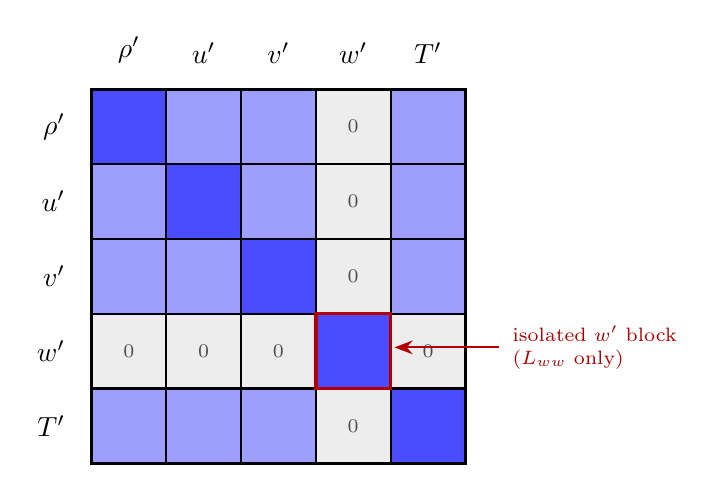
\begin{tikzpicture}[x=0.95cm,y=-0.95cm,font=\small,>=Stealth]
  \tikzset{
    nzdiag/.style={draw=black, fill=blue!70},
    nzcpl/.style={draw=black, fill=blue!38},
    zblk/.style={draw=black, fill=gray!14},
  }

  \foreach \i/\name in {0/$\rho'$,1/$u'$,2/$v'$,3/$w'$,4/$T'$} {
    \node[anchor=east,font=\bfseries] at (-0.22,\i+0.5) {\name};
    \node[anchor=south,font=\bfseries] at (\i+0.5,-0.22) {\name};
  }

  \foreach \i/\j in {0/3,1/3,2/3,4/3,3/0,3/1,3/2,3/4} {
    \path[zblk] (\j,\i) rectangle ++(1,1);
    \node[font=\scriptsize\bfseries, text=black!70] at (\j+0.5,\i+0.5) {$0$};
  }

  \foreach \i/\j in {
    0/1,0/2,0/4,
    1/0,1/2,1/4,
    2/0,2/1,2/4,
    4/0,4/1,4/2
  } {
    \path[nzcpl] (\j,\i) rectangle ++(1,1);
  }

  \foreach \k in {0,1,2,3,4} {
    \path[nzdiag] (\k,\k) rectangle ++(1,1);
  }

  \draw[very thick] (0,0) rectangle (5,5);
  \foreach \k in {1,2,3,4} {
    \draw[thick] (0,\k) -- (5,\k);
    \draw[thick] (\k,0) -- (\k,5);
  }

  \draw[very thick, red!70!black] (3,3) rectangle (4,4);
  \draw[->, thick, red!70!black] (5.45,3.45) -- (4.05,3.45);
  \node[anchor=west, align=left, text=red!70!black, font=\scriptsize] at (5.5,3.45)
    {isolated $w'$ block\\($L_{ww}$ only)};
\end{tikzpicture}
\caption{Schematic $5\times5$ block structure of the assembled LNSE operator
$\bL$ for the special case $k_z=0$. For $k_z\neq0$, the $w'$-coupling blocks
become nonzero.}
\label{fig:sparsity}
\end{figure}

\section{Discretization: SBP, curvilinear terms, BCs, and filtering}
\label{sec:discretization}

\subsection{SBP finite differences}
\label{sec:sbp}

Spatial derivatives are approximated with summation-by-parts finite-difference
operators \citep{mattsson2004summation}. In one dimension an
SBP first-derivative operator is written as
\begin{equation}
  D = H^{-1}Q,
  \qquad
  Q + Q^\top = B,
  \label{eq:sbp_property}
\end{equation}
where $H$ is a symmetric positive-definite quadrature matrix and $B$ encodes
the boundary terms. This discrete integration-by-parts structure is the basis
for the boundary treatment and the weighted adjoint relations used later in the
resolvent workflow. The implementation ships reference tables for order-$2$,
$4$, $6$, and $8$ SBP operators on structured meshes, and includes an
automatic generator for arbitrary even order. Interior stencils are computed
via the Fornberg algorithm \citep{fornberg1988generation}, while boundary
closures are determined from the accuracy conditions and the SBP constraint
\eqref{eq:sbp_property}; the free parameters that arise for orders $\ge 6$
are resolved by maximising the accuracy at the rows nearest the interior
\citep{strand1994summation}. This makes the framework extensible to
higher-order discretisations without manual coefficient transcription.

\subsection{Curvilinear coordinate transformation}
\label{sec:curvilinear}

Curvilinear and stretched meshes are treated through a mapping from
computational coordinates $(\xi,\eta)$ to physical coordinates $(x,y)$ with
Jacobian
\begin{equation}
  J = x_\xi y_\eta - x_\eta y_\xi.
  \label{eq:jacobian}
\end{equation}
The physical derivatives are related to computational derivatives by
\begin{equation}
  \pp_x = \frac{ y_\eta \pp_\xi - y_\xi \pp_\eta}{J},
  \qquad
  \pp_y = \frac{-x_\eta \pp_\xi + x_\xi \pp_\eta}{J}.
  \label{eq:curv_first}
\end{equation}
For common one-dimensional wall-normal stretching, the expressions simplify to
\begin{equation}
  D_y = \mathrm{diag}(1/y'_\eta)\,D_\eta,
  \qquad
  D_{yy}
  = \mathrm{diag}(1/{y'_\eta}^2)\,D_{\eta\eta}
  - \mathrm{diag}(y''_\eta/{y'_\eta}^3)\,D_\eta.
  \label{eq:1d_stretch}
\end{equation}

The package provides algebraic and hyperbolic-tangent stretching functions that
cluster points near a wall while maintaining smoothness. A representative
single-sided map is
\begin{equation}
  y(\eta)
  = y_{\max}\,
  \frac{1 - \tanh\!\bigl[s(1-\eta)\bigr]/\tanh(s)}
       {1 + \tanh\!\bigl[s(1-\eta)\bigr]/\tanh(s)},
  \label{eq:stretching}
\end{equation}
where $s>0$ controls the clustering intensity and $y_{\max}$ is the domain
height.

\begin{figure}[t]
\centering
\artifactinclude{width=0.70\textwidth}{figs/example_grid.png}
\caption{Representative stretched grid with wall-normal clustering controlled
by the stretching parameter $s$.}
\label{fig:example_grid}
\end{figure}

\subsection{Boundary conditions}
\label{sec:bc}

Boundary conditions are imposed through an algebraic overwrite. For homogeneous
Dirichlet conditions on degree of freedom $i$, the generalized operator pair is
overwritten as
\begin{equation}
  A_{i,:}=0,\qquad A_{:,i}=0,\qquad
  M_{i,:}=0,\qquad M_{:,i}=0,\qquad
  A_{ii}=P_{\mathrm{bc}},\qquad M_{ii}=1,
  \label{eq:dirichlet_penalty}
\end{equation}
while zero-normal-gradient conditions replace only the boundary row with the
outward normal derivative,
\begin{equation}
  L_{i,\cdot}
  = n_x D_{x,i_{\mathrm{mesh}},\cdot}
  + n_y D_{y,i_{\mathrm{mesh}},\cdot}.
  \label{eq:neumann_penalty}
\end{equation}
Sponge layers for non-reflecting boundaries are implemented as a spatially
varying diagonal damping term
$\bL \leftarrow \bL - \mathrm{diag}(\bm{\sigma}_{\mathrm{sponge}})$.

This overwrite is not the classical SBP-SAT formulation. The parameter
$P_{\mathrm{bc}}$ must balance boundary enforcement against shifted-system
conditioning, because excessively large values can stall iterative Krylov
convergence.

\subsection{Spatial filtering}
\label{sec:filtering}

High-frequency numerical oscillations are attenuated by a 10th-order implicit
Pad\'e-type filter in the framework of \citet{lele1992compact} and
\citet{visbal2002use}. The filtered solution satisfies
\begin{equation}
  \bM_f\,\bq_{\mathrm{filt}} = \bA_f\,\bq,
  \label{eq:filter_implicit}
\end{equation}
where $\bM_f$ is a symmetric tridiagonal matrix with unit diagonal and
off-diagonal entries equal to the filter parameter $\alpha_{\mathrm{flt}}$,
\begin{equation}
  \bM_f = \mathrm{tridiag}(\alpha_{\mathrm{flt}},1,\alpha_{\mathrm{flt}}),
  \label{eq:filter_Mf}
\end{equation}
and $\bA_f$ is the explicit filter operator. In two dimensions the filters are
applied sequentially along the coordinate directions,
\begin{equation}
  \bq_{\mathrm{filt}}
  = \bM_{f,y}^{-1}\,\bM_{f,x}^{-1}\,\bA_{f,x}\,\bA_{f,y}\,\bq.
  \label{eq:filter_2d}
\end{equation}
For resolvent analysis an adjoint-consistent filter pair is required so that
the discrete adjoint relation is preserved in the weighted inner product.

\section{Verification of the discrete linearized operator}
\label{sec:linearization_verification}

The coefficient matrices in \eqref{eq:lnse_matrix} were originally derived with
computer algebra, implemented in MATLAB, and then translated to Python.
Agreement with the MATLAB reference is necessary for translation fidelity, but
it cannot detect an error shared by both implementations. The assembled
operator is therefore checked against two independent references that do not
rely on the Martini derivation itself.

\paragraph{Complex-step Jacobian verification.}
The discrete nonlinear compressible Navier--Stokes residual $\bR(\bq)$ is
evaluated on the same grid and with the same SBP operators used for the
linearized system. The exact Jacobian of $\bR$ at the base flow $\bqbar$ is
then computed column-by-column through the complex-step method
\citep{squire1998using,martins2003complex}:
\begin{equation}
  \frac{\pp R_i}{\pp q_j}\bigg|_{\bqbar}
  = \frac{\mathrm{Im}\!\left[\bR(\bqbar + \mathrm{i}\epsilon\,\mathbf{e}_j)\right]}
         {\epsilon},
  \label{eq:complex_step}
\end{equation}
with $\epsilon \sim 10^{-30}$. Unlike finite differences, complex-step
derivatives avoid subtractive cancellation and can approach machine precision
provided the residual is implemented without non-analytic operations such as
\texttt{abs} or \texttt{real}.

\paragraph{Symbolic re-derivation with SymPy.}
As a complementary check, the compressible Navier--Stokes equations are
linearized from scratch with SymPy symbolic algebra. The base-flow and
perturbation quantities are declared symbolically, the substitution
$\bq = \bqbar + \epsilon \bqp$ is expanded in $\epsilon$, and the coefficient
matrices are extracted by grouping terms according to the derivative operators.
This path is particularly useful for the Sutherland-viscosity derivative terms,
which are algebraically dense and therefore prone to sign or factor mistakes.

\paragraph{Verification status.}
The verification protocol produces two summary values:
(i)~the maximum relative discrepancy from the complex-step Jacobian check, and
(ii)~the symbolic agreement status for the coefficient sub-blocks. The Martini
example-family audit reported next is kept distinct from these operator-level
checks because it addresses translation fidelity rather than independent
derivation verification.

\section{Fidelity to the released Martini example family}
\label{sec:martini_fidelity}

The external-reference audit against the released Martini MATLAB exports is the
primary fidelity check for the shipped example family. The audit is regenerated
by \path{./run_all_examples.sh}, which rewrites the Python example artifacts,
extracts all available MATLAB parity bundles under \path{tools/parity/npz/},
and emits \path{tools/parity/reports/martini_parity_latest.json} plus
\path{tools/parity/reports/martini_parity_table.csv}.

\begin{table}[t]
\centering
\scriptsize
\setlength{\tabcolsep}{4pt}
\begin{tabular}{L{3.0cm}L{1.8cm}L{6.0cm}c}
\toprule
Case & Scope & Primary automated audit metric & Status \\
\midrule
Example 0: curvilinear derivative & protocol & $\max|df_{\mathrm{py}}-df_{\mathrm{ml}}| = 6.1\times 10^{-14}$; Python and MATLAB derivatives agree to machine precision & \texttt{PASS} \\
Example 1: Blasius resolvent & direct & $\max|\Delta\sigma|/\sigma = 0.54\%$; SVD residual $\leq 2.3\times 10^{-13}$ & \texttt{PASS} \\
Example 2: jet resolvent & direct & $\max|\Delta\sigma|/\sigma = 0.20\%$; SVD residual $\leq 7.5\times 10^{-13}$ & \texttt{PASS} \\
Example 3: streaky boundary layer & temporal + spatial & Temporal eigenvalue residual $\leq 1.3\times 10^{-11}$; spatial eigenvalue residual $\leq 5.2\times 10^{-9}$ & \texttt{PASS} \\
Example 4: cavity spectra/adjoints & direct & $\max|\Delta\omega| = 5.8\times 10^{-6}$ (direct and adjoint); eigenvalue residual $\leq 5.0\times 10^{-6}$ & \texttt{PASS} \\
Example 5: paraboloid resolvent & direct & $\max|\Delta\sigma|/\sigma = 0.043\%$; SVD residual $\leq 8.5\times 10^{-13}$ & \texttt{PASS} \\
\bottomrule
\end{tabular}
\caption{Martini example-family parity audit. All six shipped examples satisfy
the current quantitative closure criteria.}
\label{tab:accuracy_gate}
\end{table}

The example family is not a substitute for independent verification;
it demonstrates that the Python translation reproduces the released MATLAB
workflows to within the stated quantitative tolerances. The figures below
show geometry, baseflow, mode, and spectrum artifacts; additional
parity-comparison panels are available under \texttt{examples/}.

\paragraph{Example 0: curvilinear derivative validation.}
This example is a geometry/discretization protocol rather than a flow-physics
case. A symmetric computational mesh is mapped to a parabolic physical domain,
and the transformed derivative operators are checked against the analytical
derivative of $\cos(x)$. Its role in the example family is to confirm that the
curvilinear metrics and discrete derivative operators behave as intended before
they are embedded in the full LNSE assembly.

\begin{figure}[t]
\centering
\artifactinclude{width=0.48\textwidth}{../examples/example_0_curvilinear_validation_baseflow.png}
\hfill
\artifactinclude{width=0.48\textwidth}{../examples/example_0_curvilinear_validation.png}
\caption{Example~0 curvilinear-derivative protocol: mesh/geometry view and
derivative-verification summary.}
\label{fig:martini_example_0}
\end{figure}

\paragraph{Example 1: Blasius boundary-layer resolvent.}
The first flow case is a compressible flat-plate boundary layer. The baseflow
panel shows the expected streamwise acceleration from the wall to the
freestream, while the resolvent summary highlights forcing/response structures
concentrated in the boundary-layer shear region. This case probes the convective-amplifier behavior of the discretized
operator in a canonical wall-bounded shear flow.

\paragraph{Example 2: axisymmetric jet resolvent.}
This case moves to an axisymmetric jet base flow. The baseflow panel makes the
jet core and surrounding shear layer explicit, and the resolvent summary shows
the leading structures supported by that shear layer. The resolvent analysis again targets input--output amplification, now in a
free-shear-flow setting with axisymmetric geometry and radial weighting in
the compressible energy norm.

\begin{figure}[t]
\centering
\artifactinclude{width=0.48\textwidth}{../examples/example_1_blasius_baseflow.png}
\hfill
\artifactinclude{width=0.48\textwidth}{../examples/example_1_blasius.png}
\par\medskip
\artifactinclude{width=0.48\textwidth}{../examples/example_2_jet_baseflow.png}
\hfill
\artifactinclude{width=0.48\textwidth}{../examples/example_2_jet.png}
\caption{Examples~1 and~2: baseflow and resolvent-summary artifacts for the
Blasius boundary layer and the axisymmetric jet.}
\label{fig:martini_examples_12}
\end{figure}

\paragraph{Example 3: streaky boundary-layer temporal and spatial analysis.}
This example introduces a streak-modulated boundary-layer base state and uses
the same discretization machinery for both temporal and spatial analyses. The
baseflow panel shows the streak modulation, the temporal panel highlights the
leading disturbance structure at fixed streamwise wavenumber, the spatial panel
shows the corresponding downstream-growing/decaying structure at fixed
frequency, and the spectral panel summarizes the two spectra together. The
physical interpretation is secondary instability of a streaky boundary layer
rather than single-frequency resolvent amplification alone.

\begin{figure}[t]
\centering
\artifactinclude{width=0.48\textwidth}{../examples/example_3_streaky_bl_baseflow.png}
\hfill
\artifactinclude{width=0.48\textwidth}{../examples/example_3_streaky_bl.png}
\par\medskip
\artifactinclude{width=0.48\textwidth}{../examples/example_3_streaky_bl_spatial.png}
\hfill
\artifactinclude{width=0.48\textwidth}{../examples/example_3_streaky_bl_spectra.png}
\caption{Example~3 streaky-boundary-layer baseflow, temporal mode, spatial
mode, and spectral summary.}
\label{fig:martini_example_3}
\end{figure}

\paragraph{Example 4: cavity direct and adjoint global modes.}
The cavity case is the global-stability example in the family. The baseflow
panel shows the recirculating cavity region and overlying shear layer. The mode
panels then separate direct and adjoint structures. Their joint interpretation
is standard in global stability: the direct mode indicates where the global
structure is expressed, while the adjoint mode indicates where the flow is most
receptive to forcing.

\begin{figure}[t]
\centering
\artifactinclude{width=0.48\textwidth}{../examples/example_4_cavity_baseflow.png}
\hfill
\artifactinclude{width=0.48\textwidth}{../examples/example_4_cavity.png}
\par\medskip
\artifactinclude{width=0.48\textwidth}{../examples/example_4_cavity_direct.png}
\hfill
\artifactinclude{width=0.48\textwidth}{../examples/example_4_cavity_adjoint.png}
\caption{Example~4 cavity baseflow and direct/adjoint global-mode views.}
\label{fig:martini_example_4}
\end{figure}

\paragraph{Example 5: paraboloid resolvent.}
The final example returns to resolvent analysis, but on a strongly curved
axisymmetric geometry obtained through a paraboloid mapping. The baseflow panel
shows the resulting speed field over the mapped geometry, while the summary
panel shows the leading forcing/response structures. Its role in the example
family is to show that the same operator/discretization machinery extends to
curved geometries without reducing the workflow to a Cartesian special case.

\begin{figure}[t]
\centering
\artifactinclude{width=0.48\textwidth}{../examples/example_5_paraboloid_baseflow.png}
\hfill
\artifactinclude{width=0.48\textwidth}{../examples/example_5_paraboloid.png}
\caption{Example~5 paraboloid baseflow and resolvent-summary artifacts.}
\label{fig:martini_example_5}
\end{figure}

\section{External validation and current case-family status}
\label{sec:external_validation}

\subsection{Oblique SWBLI benchmark: Robinet and Song}
\label{sec:song_validation}

As an external benchmark, the project uses the oblique
shock-wave/laminar-boundary-layer interaction studied by
\citet{robinet2007bifurcations} and revisited with DNS confirmation by
\citet{song2023global}. The configuration is a standard compressible global
stability benchmark: the leading eigenvalue, the instability threshold, and
the associated global mode provide a reference that is independent of the
internal Martini example family. The current Python driver and reference data
live under \path{validation/song_2023/}.

\begin{figure}[t]
\centering
\artifactinclude{width=0.82\textwidth}{../validation/song_2023/song_2023.png}
\caption{Robinet/Song oblique SWBLI validation artifact. Left: temporal
spectrum with Python (filled), MATLAB (open circles), and Song original
(squares) eigenvalues. Right: side-by-side MATLAB (top) and Python (bottom)
streamwise velocity eigenmodes for a steady (left column) and oscillatory
(right column) branch. Python modes are phase-aligned to MATLAB.}
\label{fig:song_validation_artifact}
\end{figure}

The comparison targets are the leading eigenvalue, the threshold
value reported in the source literature, and the associated mode or
spectrum overlays. Normalization conventions are stated alongside the
comparison tables.

\paragraph{Validation status.}
After correcting the input-data layout convention (the saved MATLAB-exported
fields use \texttt{(x\_index, y\_index)} ordering, which must be transposed
before entering the \texttt{(ny, nx)} mesh path), both the SciPy-assembled
and PETSc-assembled operators produce consistent eigenvalue spectra under
direct LU/MUMPS factorization. On a reduced grid, the two assembly backends
match exactly (mean nearest-MATLAB eigenvalue distance $1.37 \times 10^{-2}$,
leading-mode growth rate $\mathrm{Im}(\omega_1) = +0.0605$). On the full
$599 \times 301$ grid with the default filtered baseflow and an
over-extraction strategy (24 modes requested, 20 nearest to target retained),
the 20-mode comparison gives a mean nearest-MATLAB distance of
$1.16 \times 10^{-2}$ and a maximum of $3.01 \times 10^{-2}$. The leading
eigenvalue is $\mathrm{Im}(\omega_1) = +0.0573$, compared to the MATLAB
reference $+0.0589$ (${\approx}\,3\%$ difference). Only three matched pairs
exceed $2 \times 10^{-2}$, and the previously observed deep-damped outlier
pair is resolved by the enlarged extraction window.

Figure~\ref{fig:song_validation_artifact} shows the current Song summary
artifact: a temporal spectrum panel with Python, MATLAB, and Song original
eigenvalues overlaid, and side-by-side Python/MATLAB mode shapes for
a steady (Mode~1) and an oscillatory (Mode~2) eigenmode. The Python
eigenvectors are phase-aligned to MATLAB via a complex least-squares
projection before plotting, so that the signed contour levels are directly
comparable. All current Song stability results in this manuscript use the
same solver stack: SLEPc Krylov--Schur as the outer eigensolver, shift-invert
for spectral targeting, and direct LU factorization with MUMPS for the inner
shifted solves.

\subsection{Application-facing Case 1 status}
\label{sec:case1}

The current turbine-cascade workflow based on \citet{lui2022unsteadiness}
plays a different role from the Robinet/Song benchmark. It is not used as
the external-validation anchor; rather, it is the application case in which the
same operator, solver, and resolvent infrastructure is applied to the
project's target configuration. Because the supplied reference state is
a mean flow, the interpretation of the resulting spectra and gains follows the
mean-flow caveat stated in Section~\ref{sec:lnse}.

\begin{table}[t]
\centering
\small
\begin{tabular}{lccccc}
\toprule
Workflow & Grid & $n = 5N$ & Leading output & Wall time [s] & Peak mem [GB] \\
\midrule
Temporal EVP & $N_x \times N_y$ & pending & $\omega_1 =$ pending & pending & pending \\
Resolvent    & $N_x \times N_y$ & pending & $\sigma_1 =$ pending & pending & pending \\
\bottomrule
\end{tabular}
\caption{Case~1 reporting template. Numerical entries are placeholders
pending completion of the reproducible artifact pipeline.}
\label{tab:case1}
\end{table}

\subsection{Application-facing Case 2 status: suction-side SWBLI}
\label{sec:case2}

The Case~2 configuration is the oblique shock-wave/boundary-layer
interaction on the suction side of the supersonic turbine cascade of
\citet{lui2022unsteadiness}: a real-gas ($\gamma = 1.31$,
$T_0 = 1540\,\text{K}$) flow at $\mathrm{Re}=3.95\times 10^5$,
$\mathrm{Ma}=2.0$, $\mathrm{Pr}=0.747$. The reference state is the
time and spanwise average of Lui's LES. Unlike Case~1, Case~2 has
two compounding non-idealities (Sec.~\ref{sec:lnse}): it is a mean
flow rather than a fixed point, and the $\gamma$ used in the
linearized operator differs from the $\gamma=1.4$ of the upstream
LES. Both are accepted as deliberate trade-offs for physical realism
of the linear analysis; their consequences are made visible in the
results below rather than hidden.

\paragraph{Mesh and operator.} The native mesh is curvilinear
body-fitted, $679$ wall-normal $\times$ $599$ streamwise cells. We
denote by \texttt{M1} the native mesh and by \texttt{M2} its
symmetric $(2,2)$-stride coarsening ($340 \times 300$, operator size
$n = 5.10\times 10^5$). Asymmetric stride coarsenings are not used:
in a body-fitted mesh around a curved wall they produce cells with a
location-dependent physical aspect ratio, which is not a natural
coarsening of the physical problem. Only uniform decimation
preserves the body-fitted interpretation.

\paragraph{Mean-flow characterisation.} The raw Lui mean flow
$\bar{Q}_{\text{raw}}$ carries a sharp oblique-shock system. The
two-dimensional spatial FFT of the streamwise velocity component
shows energy along two diagonal ridges in $(k_\xi, k_\eta)$ space
extending past the \texttt{M2} Nyquist box to the native Nyquist
boundary (Fig.~\ref{fig:case2_baseflow_fft}). The wall-normal gradient
$|\partial \bar{u}/\partial \eta|$ attains its maximum at the first
interior cell next to the Dirichlet wall, and the streamwise
gradient $|\partial \bar{u}/\partial \xi|$ attains its maximum at
the shock foot on the wall, $(x, y) \approx (0.815, -0.092)$.

\begin{figure}[t]
\centering
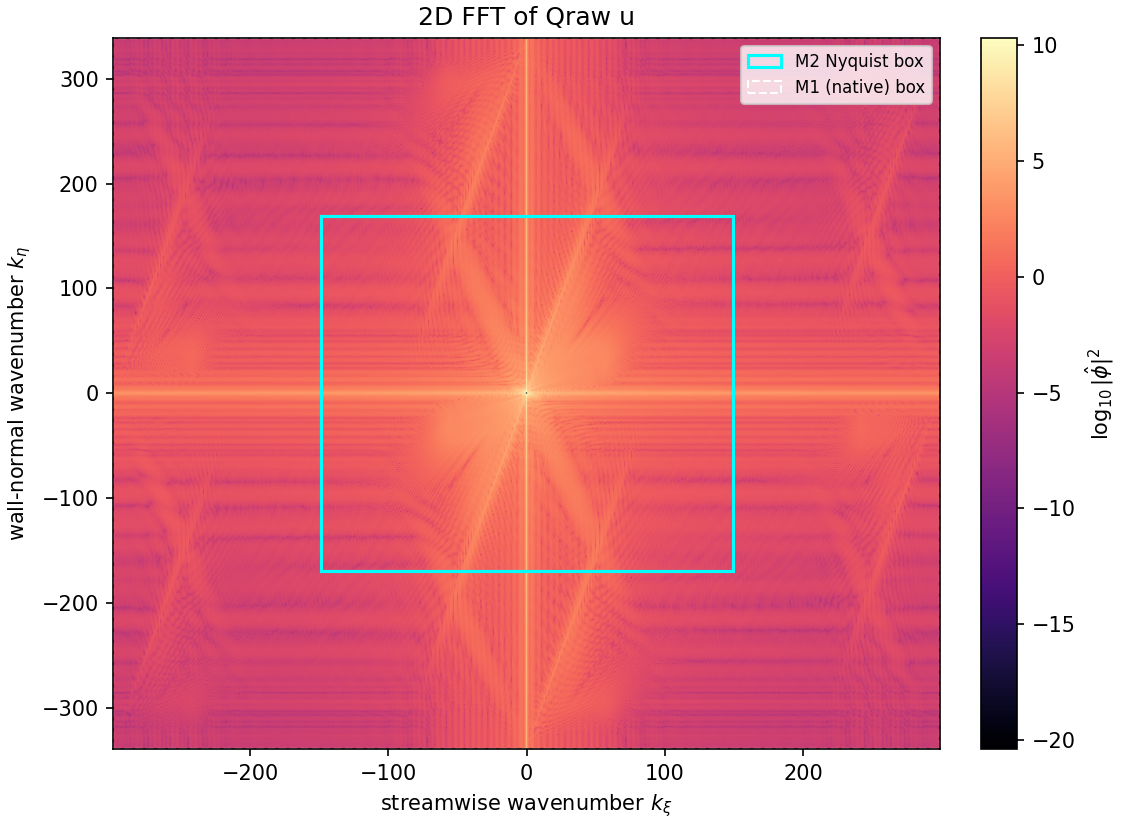
\includegraphics[width=0.85\textwidth]{../results/case2/phase1p5/qraw_u_2d_fft.png}
\caption{Two-dimensional FFT of the Case~2 streamwise mean velocity
$\bar{u}(\xi, \eta)$ on \texttt{M2}. Diagonal shock ridges extend
past the cyan \texttt{M2} Nyquist box to the native \texttt{M1}
boundary.}
\label{fig:case2_baseflow_fft}
\end{figure}

\paragraph{Temporal EVP spectrum on \texttt{M2}.} Using SLEPc
Krylov--Schur with shift-invert and MUMPS direct inner solves at
target $\omega_\sigma = -0.83\mathrm{i}$, we obtain $>60$ converged
Ritz values at $\text{eps\_tol}=5\times 10^{-3}$ (baseline screening).
A focused topology probe around candidate shock-breathing
frequencies enriches the set to $\sim 120$ classified eigenvalues
(Fig.~\ref{fig:case2_spectrum}). Each eigenmode is classified by its
compressible (Chu 1965) energy localisation: \textsc{wall-local} if
more than $30\%$ of the $E_{\text{Chu}}$ sits in the near-wall strip
or within a disk of radius $0.08$ around the shock foot;
\textsc{global} if the spatial extent (fraction of grid cells with
$E_{\text{Chu}} > 1\% \cdot \max$) exceeds $20\%$ and the wall
fraction is below $30\%$; \textsc{intermediate} otherwise.

\begin{figure}[t]
\centering
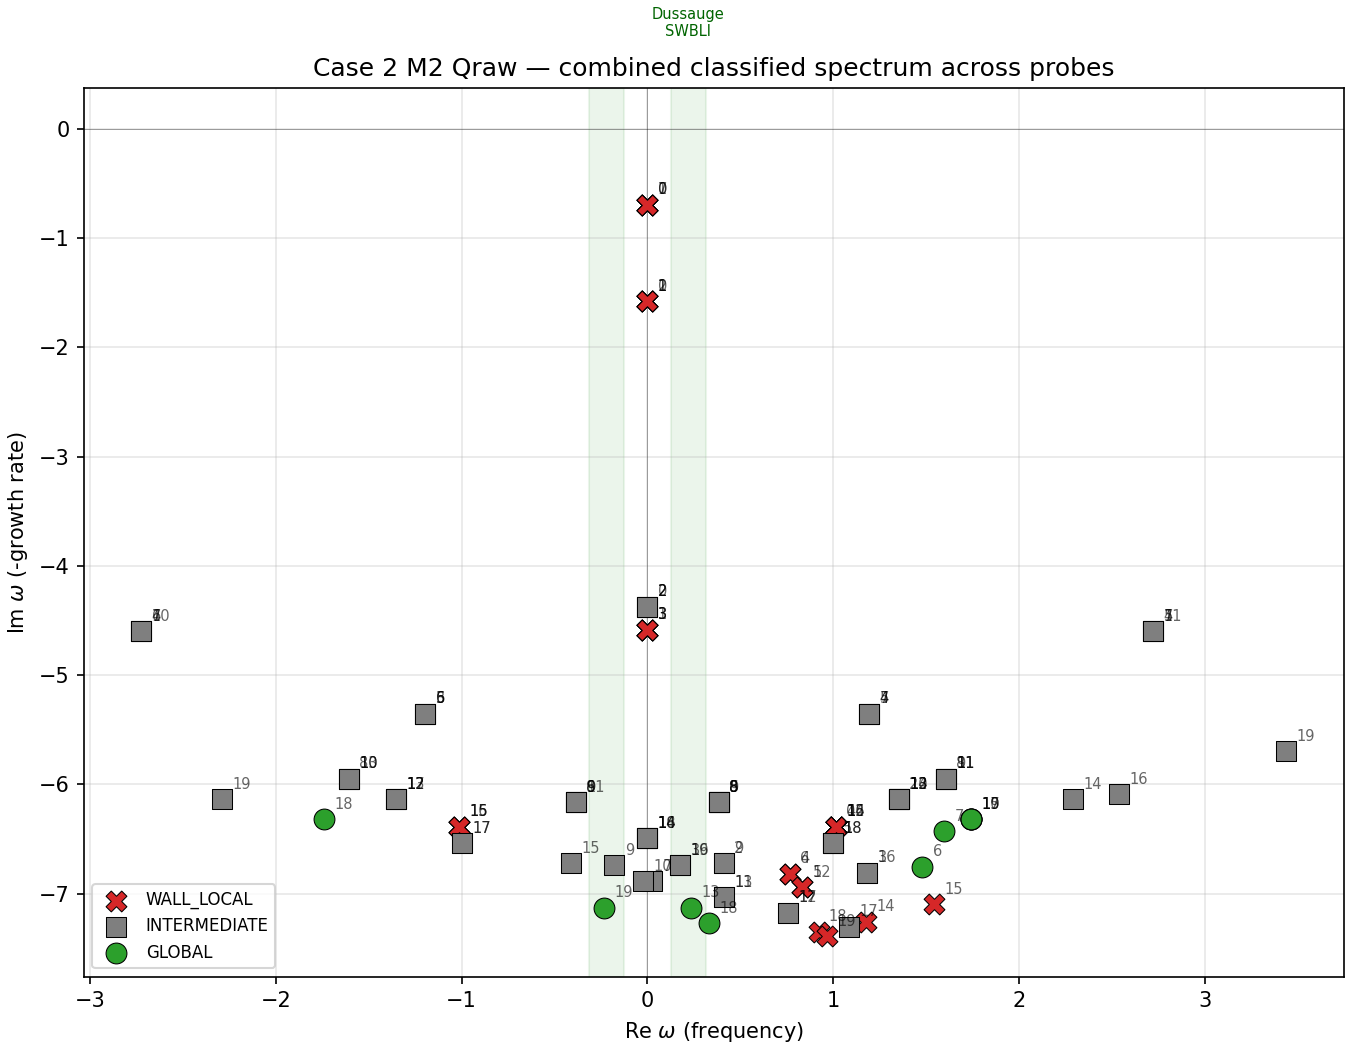
\includegraphics[width=0.9\textwidth]{../results/case2/phase1p5/combined_classified_spectrum.png}
\caption{Case~2 \texttt{M2} classified temporal EVP spectrum of
$\bar{Q}_{\text{raw}}$, combining a $\texttt{nev}=20$ screening at
two targets with a four-target focused topology probe
(120~eigenvalues total). Red crosses mark \textsc{wall-local}
contamination modes (shock-foot / near-wall Chu energy dominated).
Green disks mark \textsc{global} oscillatory modes. Grey squares
are \textsc{intermediate}. The shaded vertical bands indicate the
SWBLI low-frequency Strouhal range typical of the experimental
and high-fidelity simulation literature on unsteady shock--boundary
layer interaction \citep{lui2022unsteadiness}.}
\label{fig:case2_spectrum}
\end{figure}

Key qualitative features of Fig.~\ref{fig:case2_spectrum}:

\begin{itemize}
\item \textbf{Wall-local cluster on the imaginary axis.} The modes
  closest to $\omega = 0$ (e.g.\ $\omega = -0.695\mathrm{i}$ and
  $\omega = -1.578\mathrm{i}$) are wall-local, with peak spatial
  structure coincident within one cell of the $|\partial
  \bar{u}/\partial x|$ or $|\partial \bar{u}/\partial y|$ maxima.
  They are the direct expression of the mean-flow-gradient
  inflation at the shock foot and recovery wall.
\item \textbf{Damped oscillatory branch.} At $\mathrm{Im}(\omega)
  \approx -6$ to $-7$ we recover a band of oscillatory conjugate
  pairs at $|\mathrm{Re}(\omega)| \in [0.23, 1.74]$. The
  \textsc{global}-classified pair at
  $\omega \approx (\pm 0.235, -7.129\mathrm{i})$ corresponds to
  $\mathrm{St} \approx 0.037$, which sits inside the Dussauge
  SWBLI low-frequency range; its peak is in the recovery-zone
  freestream at $(x,y)\approx(1.08, 0.17)$, consistent with a
  globally extended cavity response rather than wall-trapped
  contamination.
\item \textbf{No resonantly unstable mode on M2.} All $120$ classified
  eigenvalues have $\mathrm{Im}(\omega) < 0$. An apparent unstable
  eigenvalue at $\omega = +3.17\mathrm{i}$ that we observed
  transiently on an earlier asymmetric-stride mesh did not survive
  the transition to symmetric \texttt{M2}; it was a discretisation
  artefact of the non-uniform coarsening.
\end{itemize}

\paragraph{Resolvent gain on \texttt{M2}.} At $\beta=0$ we compute
the leading three singular values of $(\mathrm{i}\omega I -
L_{\bar{Q}})^{-1}$ in the Chu inner product for
$\omega \in [0.10, 3.00]$, spanning the Dussauge SWBLI range and
the three $|\mathrm{Re}(\omega)|$ locations of the
\textsc{global}-classified EVP modes
(Fig.~\ref{fig:case2_gain_curve}).

\begin{figure}[t]
\centering
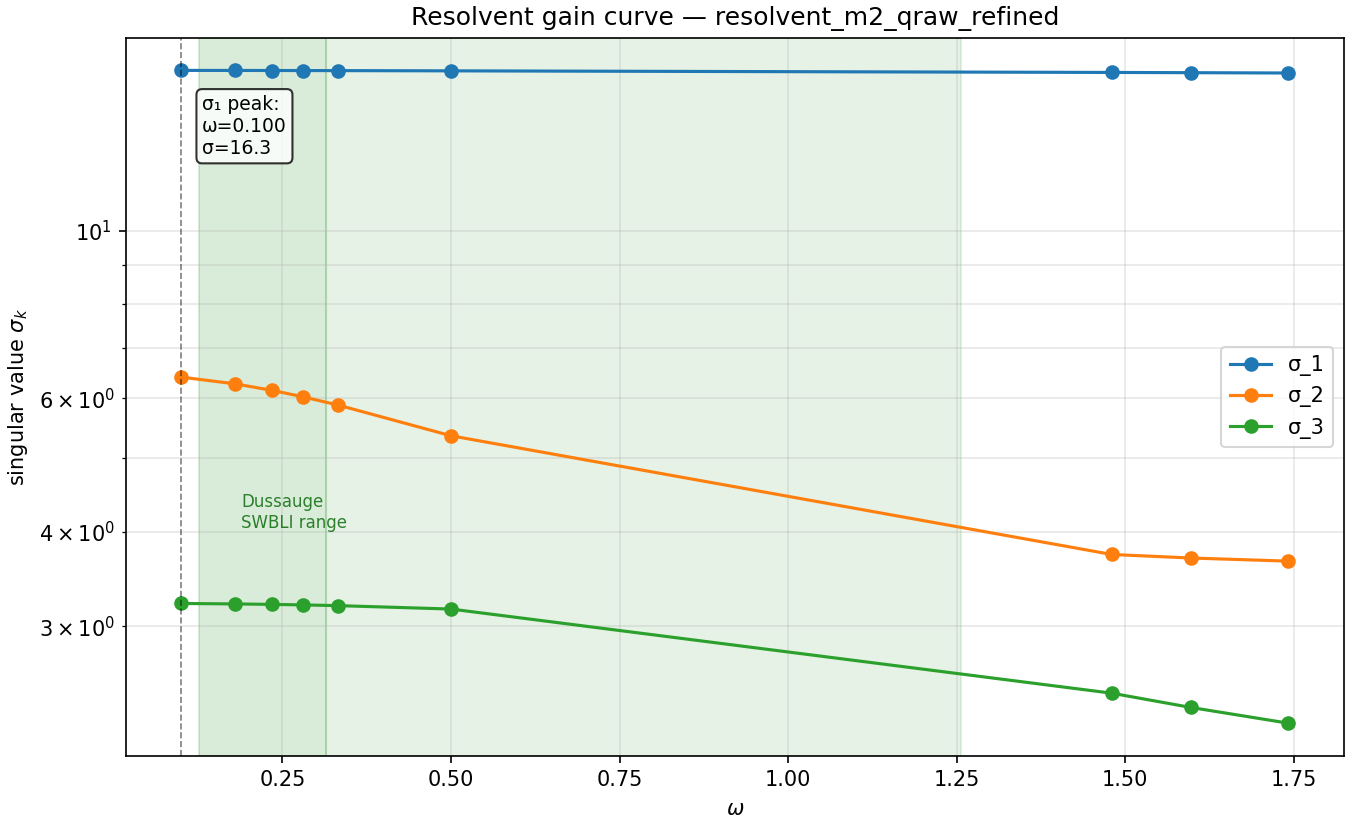
\includegraphics[width=0.88\textwidth]{../results/case2/phase1p5/resolvent_resolvent_m2_qraw_refined_gain_curve.png}
\caption{Case~2 \texttt{M2} resolvent gain $\sigma_k(\omega)$ for
$k=1,2,3$ on $\bar{Q}_{\text{raw}}$. The primary gain $\sigma_1$
is nearly independent of $\omega$; the subdominant gains
$\sigma_2, \sigma_3$ decay monotonically over the range.}
\label{fig:case2_gain_curve}
\end{figure}

Two observations frame the interpretation:

\begin{enumerate}
\item $\sigma_1(\omega) \simeq 16.27$ to within $0.8\%$ across a
  seventeen-fold frequency range, and is unchanged at the
  \textsc{global}-mode positions $\omega \in \{0.235, 0.333, 1.742\}$
  relative to adjacent non-resonant $\omega$. This is not a modal
  resonance on any individual eigenvalue; it is the ${\varepsilon}$-
  pseudospectral gain of a strongly non-normal operator in the
  Trefethen--Embree sense \citep{trefethen2005spectra}.
\item The leading optimal forcing is a narrow structure localised at
  the shock foot; the leading optimal response is a diagonal
  shock-band pattern across the domain, and both are $\omega$-
  invariant in shape (Fig.~\ref{fig:case2_fr_modes}). The
  subdominant $\sigma_2(\omega)$ drops from $6.40$ at $\omega=0.10$
  to $3.66$ at $\omega=1.74$; its response has a more distributed
  character that does depend on $\omega$.
\end{enumerate}

\begin{figure}[t]
\centering
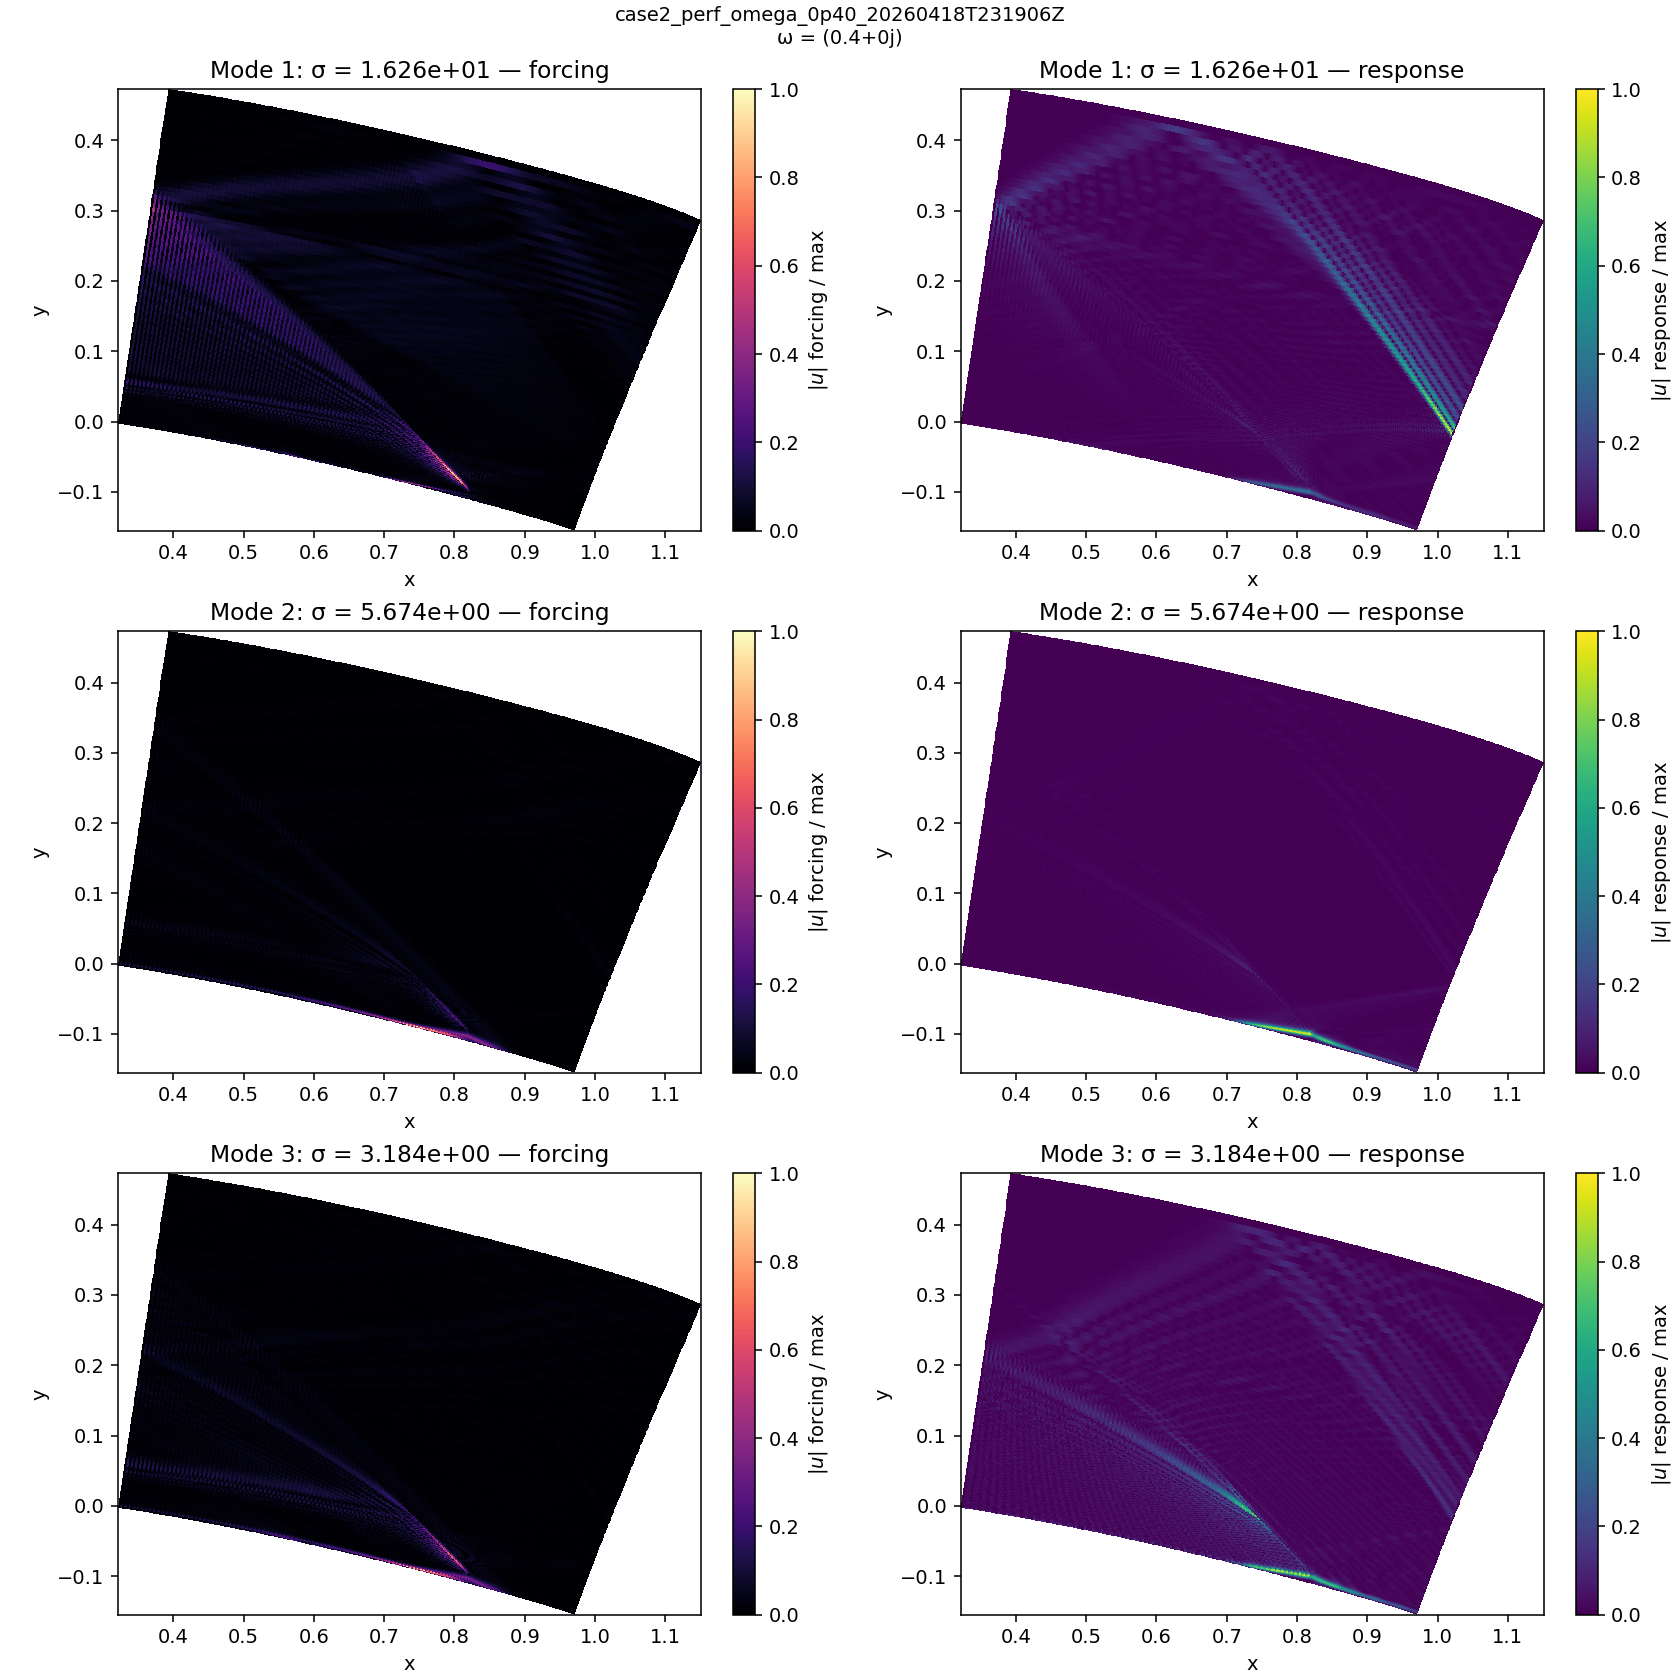
\includegraphics[width=0.95\textwidth]{../results/case2/phase1p5/case2_perf_omega_0p40_20260418T231906Z_fr_modes.png}
\caption{Optimal forcing (left column) and optimal response (right
column) structures of the three leading resolvent modes at
$\omega=0.40$ on Case~2 \texttt{M2}. The primary pair is localised
at the shock foot (forcing) and in the diagonal shock band
(response).}
\label{fig:case2_fr_modes}
\end{figure}

\paragraph{Interpretation: two amplification regimes.} Together
Figs.~\ref{fig:case2_spectrum}--\ref{fig:case2_fr_modes} split the
Case~2 amplification into:

\begin{itemize}
\item A \textbf{broadband pseudospectral regime} controlled by the
  mean-flow-gradient inflation at the shock foot and the
  recovery-zone wall, visible as the flat $\sigma_1(\omega)$ and
  the wall-local EVP cluster. This regime is a direct signature of
  the DNS-operator on LES-mean consistency gap discussed in
  Sec.~\ref{sec:lnse}.
\item A \textbf{frequency-selective modal regime} with damped
  oscillatory conjugate pairs spread over $\omega \in [0.2, 1.8]$
  and $\mathrm{Im}(\omega) \in [-7, -5]$, some of which sit inside
  the Dussauge SWBLI low-frequency range and project on globally
  extended cavity-shaped responses.
\end{itemize}

Route-3 mean-flow filtering (see Sec.~\ref{sec:lnse}) is expected to
reduce the broadband-regime contribution; the comparison on a
filtered mean-flow variant $\bar{Q}_{\text{filt}}$ from the upstream
LES pipeline is an active companion study, outside the scope of this
manuscript.

\paragraph{Cross-mesh verification.} A single \texttt{M1} stationary-
target EVP case ($n = 2.03\times 10^6$) returns
$\omega \approx \pm 0.084 - 0.536\mathrm{i}$, differing from
\texttt{M2} at the same target (Mode~0 at $\omega = -0.695\mathrm{i}$)
by $23\%$ in $|\omega|$. The qualitative near-stationary-axis cluster
survives refinement, but specific eigenvalues do not. A \texttt{M1}
resolvent check at $\omega = 0.4$ required more than an hour of
MUMPS direct factorisation and was not completed within the
present compute budget; verifying mesh-independence of $\sigma_1
\simeq 16.27$ on \texttt{M1} is left to the PETSc-iterative Strategy~B
workflow (Sec.~\ref{sec:solvers}).

\section{Harmonic-resolvent formulation and extension}
\label{sec:harmonic_extension}

Classical resolvent analysis linearizes about a steady base or mean flow. When
the dominant dynamics involve a time-periodic reference state or strong
cross-frequency coupling, a steady-base resolvent may not capture the full
amplification structure. This is the motivation for the harmonic-resolvent
framework developed by \citet{padovan2020harmonic} and extended to subharmonic
settings by \citet{padovan2022subharmonic}.

The core construction is still operator-based. Let the time-periodic base flow
have fundamental frequency $\omega_0$, and expand the perturbation on a finite
harmonic set. The resulting harmonic operator has the schematic block form
\begin{equation}
  \bL_{\mathrm{harm}} =
  \begin{bmatrix}
    \ddots & \vdots & \ddots \\
    \cdots & \bL_0 - \mathrm{i}k\omega_0 \bI & \cdots \\
    \ddots & \vdots & \ddots
  \end{bmatrix},
\end{equation}
with off-diagonal blocks carrying the cross-frequency coupling induced by the
periodic base flow. Classical resolvent is therefore recovered as the
steady-base limit of the broader harmonic formulation.

For LinStabPy, the main architectural implication is that harmonic resolvent
should not be treated as an unrelated downstream script. It is another
operator-level analysis that reuses the same physics-specific assembly while
extending the operator to multiple harmonics. This motivates an explicit
operator layer in the software design and a solver layer that can host direct,
iterative, shell-based, or randomized harmonic workflows without changing the
physical assembly interface.

In practice, harmonic-resolvent calculations require explicit choices for the
retained harmonic set, truncation level, weighting strategy, and the reference
state itself (periodic base flow versus mean-based surrogate). These choices
are exposed as configuration parameters in the implementation.

\section{Solver configurations, preconditioners, and performance}
\label{sec:solvers}

\subsection{Solver architecture}
\label{sec:design}

The dominant computational cost of the analyses described above is repeated
solution of large sparse shifted non-Hermitian systems:
$(\bL - \sigma \bM)\bx = \bb$ for eigenvalue problems and
$(\bL + \mathrm{i}\omega \bM)\bx = \bb$ for resolvent analysis. PETSc provides
a unified interface for sparse matrices, iterative or direct linear solvers,
and preconditioning, while SLEPc supplies the eigensolver and spectral
transformation layers \citep{balay2025petsc,hernandez2005slepc}. The current
default path assembles the operator in SciPy sparse format and converts it once
to a PETSc AIJ matrix.

\begin{figure}[t]
\centering
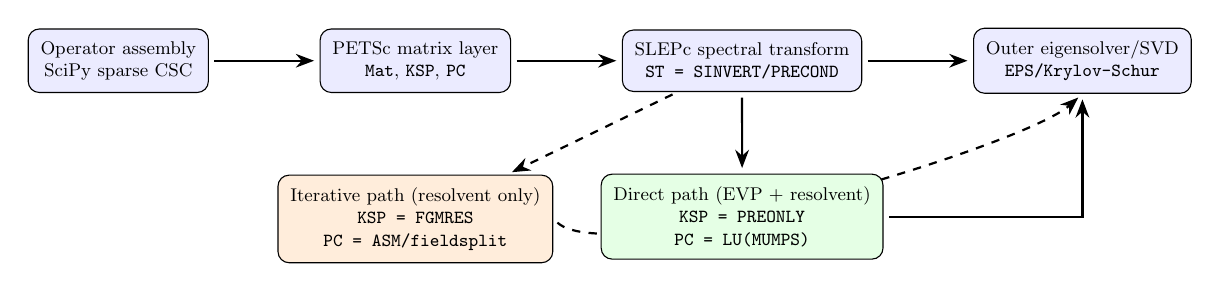
\begin{tikzpicture}[
    node distance=1.8cm and 1.9cm,
    inner sep=6pt,
    outer sep=auto,
    font=\small,
    align=center,
    scale=0.74,
    every node/.style={transform shape},
    >=Stealth,
    shorten >=2pt,
    shorten <=2pt,
    core/.style={rectangle, rounded corners, draw, minimum width=3.0cm, minimum height=1.0cm, fill=blue!8},
    patha/.style={rectangle, rounded corners, draw, minimum width=3.2cm, minimum height=1.0cm, fill=green!10},
    pathb/.style={rectangle, rounded corners, draw, minimum width=3.2cm, minimum height=1.0cm, fill=orange!14}
]
  \begin{pgfonlayer}{foreground}
  \node[core] (asm) {Operator assembly\\SciPy sparse CSC};
  \node[core, right=of asm] (petsc) {PETSc matrix layer\\\texttt{Mat}, \texttt{KSP}, \texttt{PC}};
  \node[core, right=of petsc] (st) {SLEPc spectral transform\\\texttt{ST = SINVERT/PRECOND}};
  \node[core, right=of st] (outer) {Outer eigensolver/SVD\\\texttt{EPS/Krylov-Schur}};

  \node[patha, below=1.4cm of st] (a) {Direct path (EVP + resolvent)\\\texttt{KSP = PREONLY}\\\texttt{PC = LU(MUMPS)}};
  \node[pathb, below=1.4cm of petsc] (b) {Iterative path (resolvent only)\\\texttt{KSP = FGMRES}\\\texttt{PC = ASM/fieldsplit}};
  \end{pgfonlayer}

  \draw[->, thick] (asm) -- (petsc);
  \draw[->, thick] (petsc) -- (st);
  \draw[->, thick] (st) -- (outer);
  \draw[->, thick] (st) -- (a);
  \draw[->, thick, dashed] (st) -- (b);
  \draw[->, thick] (a.east) -| (outer.south);
  \draw[->, thick, dashed] (b.east) .. controls +(1.0,-0.9) and +(-1.0,-0.9) .. (outer.south);
\end{tikzpicture}
\caption{Solver architecture of the current \texttt{linstabpy} implementation.
The assembled operator is converted to PETSc once, after which the eigensolver
and resolvent workflows operate through PETSc/SLEPc.}
\label{fig:architecture}
\end{figure}

\subsection{Direct and iterative strategies}
\label{sec:iterative}

Two solver strategies are exposed. The \emph{direct path} is a MUMPS
sparse-direct baseline used for both eigenvalue problems and resolvent
analysis:
\begin{itemize}[nosep]
  \item \textbf{Direct solver:} factor the shifted sparse matrix once, then
    apply forward/back substitutions for each right-hand side.
\end{itemize}
For the current Song stability calculations, this direct path appears inside
the SLEPc shift-invert eigensolver: the outer algorithm is Krylov--Schur,
while each shifted linear system is handled by direct LU/MUMPS.
The \emph{iterative path} is a Krylov/preconditioner route currently used only
for the resolvent linear solves:
\begin{itemize}[nosep]
  \item \textbf{Iterative solver:} build successive approximations using
    Krylov matrix-vector products and a preconditioner until the residual
    tolerance is met.
\end{itemize}
In the current implementation, the iterative route is built around
ASM/domain-decomposition preconditioners; for the algorithmic background of
these methods, see \citet{dolean2015introduction}.

\paragraph{Remark: iterative inner solvers for eigenvalue problems.}
The code infrastructure allows an iterative KSP to replace the direct solver
inside the SLEPc shift-invert spectral transformation. Systematic testing on
the Martini example family has shown that lightweight preconditioners (ASM,
block-Jacobi, ILU, Jacobi) diverge on all tested cases, and that GMRES with
an exact LU preconditioner is the only iterative configuration that converges
on the reduced Example~3 and Example~4 operators. Because even the LU-
preconditioned iterative path has not yet been validated on harder cases,
the eigenvalue path uses only the direct solver at present. See
Section~\ref{sec:krylov_roles} for a discussion of the distinction between
inner and outer Krylov strategies and the role of shifted-system conditioning.

\begin{table}[t]
\centering
\small
\setlength{\tabcolsep}{5pt}
\begin{tabular}{L{2.8cm}L{4.4cm}L{4.4cm}}
\toprule
Criterion & Direct path: MUMPS sparse-direct & Iterative path: preconditioned Krylov \\
\midrule
Core mechanism & Sparse LU factorization once, then triangular solves for each right-hand side. & Iterative residual reduction with matrix-vector products and preconditioner applications. \\
Robustness & High robustness for difficult non-normal shifted systems. & Dependent on preconditioner quality and shift conditioning. \\
Memory profile & Higher memory demand due to fill-in and factor storage. & Lower memory footprint because no global LU factors are formed. \\
Setup cost & Potentially high one-time factorization cost. & Lower setup cost, but solve cost depends on iteration count. \\
Repeated solves & Efficient after factorization, especially for many solves at fixed shift. & Cost scales with the inner-iteration history and can vary across shifts/frequencies. \\
Current scope & Used for all eigenvalue problems and as the resolvent default. & Used for resolvent analyses only; not yet validated for the shift-invert eigensolver inner loop. \\
\bottomrule
\end{tabular}
\caption{Comparison of the two solver strategies. The iterative path is
currently used only for resolvent analyses; see the remark in
Section~\ref{sec:iterative} regarding eigenvalue-problem limitations.}
\label{tab:direct_iterative_compare}
\end{table}

\begin{table}[t]
\centering
\footnotesize
\setlength{\tabcolsep}{4pt}
\begin{tabular}{L{1.7cm}L{2.7cm}L{2.8cm}L{3.0cm}L{3.2cm}}
\toprule
Layer & Option pattern & Default role & Why chosen & When to change \\
\midrule
SLEPc & $ST=$ SINVERT & Interior-target extraction & Maps target eigenvalues to dominant transformed eigenpairs & Change shift $\sigma$ when the target region moves \\
PETSc KSP/PC & PREONLY + LU(MUMPS) & EVP and resolvent direct inner solve & Necessary for the non-normal shifted LNSE systems encountered in practice & Replace only after validating an iterative alternative on the target case \\
PETSc KSP/PC & FGMRES + ASM & Resolvent iterative solve & Flexible Krylov route for variable preconditioning quality & Adjust overlap or preconditioner family when convergence stalls \\
Conv. guard & \path{ksp_error_if_not_converged} & Hard failure semantics & Prevents polluted outer spectra from unconverged inner solves & Do not disable for production claims \\
\bottomrule
\end{tabular}
\caption{Solver-option rationale for the current PETSc/SLEPc configuration
layer.}
\label{tab:solver_rationale}
\end{table}

The solver-selection workflow is intentionally explicit:
\begin{enumerate}[label=\arabic*., nosep]
  \item assemble and validate the operator on the target grid;
  \item use the direct path (PREONLY + LU/MUMPS) for all eigenvalue problems;
  \item for resolvent analyses, use the direct path as the reference, then
    switch to the iterative path when memory or distribution constraints make
    direct factorization impractical;
  \item compare iterative resolvent outputs against a nearby direct-path
    reference case before scaling up;
  \item reject production results when inner linear solves fail their
    prescribed tolerances.
\end{enumerate}

\subsection{Matrix-forming versus time-stepper Krylov strategies}
\label{sec:krylov_roles}

A point of frequent confusion in the stability-analysis literature is the role
of Krylov methods. The term ``Krylov'' appears in two distinct contexts that
share mathematical foundations but differ in their numerical requirements and
failure modes. Because LinStabPy is a matrix-forming code, this distinction
directly determines the solver architecture.

\paragraph{Outer Krylov: the time-stepper approach.}
In the time-stepper formulation
\citep{edwards1994krylov,barkley2008direct,frantz2023krylov}, the linearized
operator $\bL$ is never assembled. Instead, the action of the propagator
$\mathrm{e}^{\bL \Delta t}$ (or an approximation to it) is evaluated by
advancing the linearized equations one time step. The Arnoldi algorithm builds
a Krylov basis $\{\bv, \mathrm{e}^{\bL\Delta t}\bv,
(\mathrm{e}^{\bL\Delta t})^2 \bv, \ldots\}$ and extracts the dominant
eigenvalues of the propagator, which correspond to the least-stable temporal
modes \citep{lehoucq1998arpack}. No matrix is stored, no system is inverted,
and the Arnoldi recurrence operates on the smooth output of the time-stepper.
This is the approach used by spectral-element codes such as Nek5000 and
Nektar++, and by operator-free resolvent tools such as
\texttt{LightKrylov}~\citep{kern2026lightkrylov}.

\paragraph{Inner Krylov: iterative shift-invert.}
When a matrix-forming code needs interior eigenvalues near a target $\sigma$,
the standard technique is the shift-invert spectral transformation:
the eigensolver (Krylov--Schur in SLEPc) repeatedly applies
$(\bL - \sigma\bI)^{-1}$ to Arnoldi vectors
\citep{hernandez2005slepc,lehoucq1998arpack}. Each application requires
solving the shifted linear system $(\bL - \sigma\bI)\bx = \bb$. With a
direct solver (LU/MUMPS) this reduces to forward/back substitutions using
a precomputed factorization. If instead an iterative Krylov method (e.g.\
GMRES) is used for these inner solves, it must invert the shifted operator
to high accuracy at every outer Arnoldi step. The current Song runs use the
former configuration: outer Krylov--Schur with direct LU/MUMPS inner solves,
not GMRES/ASM or another iterative inner KSP.

\paragraph{Why the inner solve is demanding for compressible LNSE.}
The shifted temporal operator $\mathrm{i}\bL - \sigma\bI$ inherits the
non-normality of the linearized Navier--Stokes equations. For compressible
flows, the LNSE operator couples five thermodynamic variables with disparate
scales and supports convective non-normality
\citep{trefethen1993hydrodynamic,schmid2007nonmodal} as well as
continuous-spectrum modes near the real axis. When the spectral target
$\sigma$ lies near the continuous spectrum or a cluster of eigenvalues, the
shifted operator can become poorly conditioned
\citep{trefethen2005spectra,saad2003iterative}.

The practical consequences were observed in the Martini example family.
On reduced grids of Example~3 (streaky boundary layer) and Example~4
(cavity), a systematic sweep of ten Krylov/preconditioner configurations
found that only GMRES with an exact LU preconditioner (\texttt{gmres +
lu}, right-preconditioned) converges; all lightweight preconditioners (ASM,
block-Jacobi, ILU, Jacobi, fieldsplit) diverged
(\texttt{KSP\_DIVERGED\_ITS}, 20\,000~iterations). This indicates that the
inner shifted solve requires a preconditioner that closely approximates the
inverse of the shifted operator --- local or incomplete approximations are
insufficient for the non-normal compressible LNSE.

For the direct path (\texttt{PREONLY} + LU/MUMPS), the outer Krylov--Schur
iteration checks only the \emph{eigenpair} residual, not the inner
linear-system residual. The direct solve therefore succeeds even on shifted
systems where the inner-solve accuracy would be marginal for an iterative
method, because the outer eigensolver tolerates moderate perturbations in
the search directions.

\paragraph{Implications for solver selection.}
The distinction between outer and inner Krylov roles leads to a practical
guideline:
\begin{itemize}[nosep]
\item \emph{Matrix-forming codes} (including LinStabPy): use direct
  factorization for the shift-invert inner solves. The formed matrix enables
  exact factorization, which decouples the outer eigenvalue convergence from
  inner-solve accuracy. This is the default and currently the only validated
  EVP path.
\item \emph{Time-stepper / matrix-free codes}: use the outer Krylov approach
  on the propagator. No inner linear system is formed or inverted; the
  non-normality is encoded in the time-stepper output, which the outer
  Arnoldi handles without shift-invert.
\item \emph{Resolvent analysis}: both paths are viable. The resolvent requires
  solving a single shifted system $(\bL + \mathrm{i}\omega\bI)\bx = \bb$
  rather than embedding the solve inside an outer eigenvalue loop. The
  accuracy requirement is therefore that of a one-shot linear solve, which is
  less demanding than the repeated inner solves needed by shift-invert.
  Iterative Krylov with domain-decomposition preconditioning (FGMRES + ASM)
  may therefore succeed for resolvent even when it fails for eigenvalue
  problems.
\end{itemize}
These observations are consistent with the broader experience reviewed by
\citet{theofilis2011global} and \citet{frantz2023krylov}: the choice between
matrix-forming and time-stepper approaches is not simply a matter of
preference but determines which solver strategies are available and where
non-normality enters the computation.

\subsection{Performance structure}
\label{sec:scaling}

Performance reporting is organized around wall time, peak memory, solver
configuration, and hardware metadata.

\begin{table}[t]
\centering
\small
\begin{tabular}{lccccc}
\toprule
 & & \multicolumn{4}{c}{Serial, direct LU/MUMPS} \\
\cmidrule(lr){3-6}
Order & DOF ($5N$) & Assemble [s] & Solve [s] & Total [s] & Peak [GB] \\
\midrule
fd2 & 901\,495 & pending & pending & pending & pending \\
fd4 & 901\,495 & pending & pending & pending & pending \\
fd6 & 901\,495 & pending & pending & pending & pending \\
fd8 & 901\,495 & pending & pending & pending & pending \\
\bottomrule
\end{tabular}
\caption{Song 2023 oblique SWBLI benchmark on the $599\times301$ grid:
assembly and eigensolve cost versus finite-difference order. All runs are
serial (1~MPI rank) with PETSc local assembly and MUMPS direct
factorisation. The DOF count is constant because all orders share the same
grid; only the stencil bandwidth changes.}
\label{tab:scaling}
\end{table}

\section{Reproducibility and code map}
\label{sec:repro_checklist}

The supplement keeps the paper-to-code map explicit so that each main equation
or workflow can be traced to the implementation entry point.

\begin{table}[t]
\centering
\small
\begin{tabular}{L{1.3cm}L{3.1cm}L{4.1cm}L{3.7cm}}
\toprule
Eq. & Description & File & Entry point \\
\midrule
(\ref{eq:lnse_matrix}) & LNSE matrix form & \path{operators/coefficients.py} & \path{LNSECoefficients} \\
(\ref{eq:gevp})--(\ref{eq:shift_invert}) & Temporal EVP & \path{solvers/eigenvalue.py} & \path{temporal_eigenvalues} \\
(\ref{eq:adjoint_op}) & Adjoint operator & \path{solvers/eigenvalue.py} & \path{adjoint_eigenvalues} \\
(\ref{eq:qep})--(\ref{eq:companion}) & Spatial EVP / companion form & \path{operators/spatial.py} & \path{build_spatial_operator} \\
(\ref{eq:weighted_svd}) & Resolvent SVD & \path{solvers/resolvent.py} & \path{resolvent_analysis} \\
(\ref{eq:chu_norm})--(\ref{eq:W_diag}) & Chu energy norm & \path{operators/energy_norm.py} & \path{build_energy_norm} \\
(\ref{eq:floquet_shift}) & Floquet shift & \path{operators/assembly.py} & \path{assemble_lnse} \\
(\ref{eq:filter_implicit})--(\ref{eq:filter_2d}) & Implicit filter & \path{mesh/filters.py} & \path{build_filter} \\
\bottomrule
\end{tabular}
\caption{Mapping of the main supplementary equations to the implementation
entry points under \texttt{src/linstab2d/}.}
\label{tab:eq_code_map}
\end{table}

Two command paths are kept separate on purpose.

For the external-reference Martini audit, the canonical command is
\begin{verbatim}
./run_all_examples.sh
\end{verbatim}
which regenerates the comparison-eligible example outputs and refreshes the
JSON/CSV audit reports under \path{tools/parity/reports/}.

For the current Case~1 workflow, the repository command path remains the
case-specific driver under \path{results/case1/}. The paper-facing artifacts
should be sourced from that workflow rather than copied into the supplement by
hand.

\paragraph{Code availability.}
LinStabPy is available at \url{https://github.com/ricardofrantz/linstabpy} as
the Python package \texttt{linstabpy}; release DOI and snapshot metadata will
be added in the final submission package.

\bibliographystyle{unsrtnat}
\bibliography{refs}

\end{document}
